\chapter{Desarrollo de un software de análisis de trazabilidad de tiempo}

\section{Introducción}

Como se describe en los objetivos del trabajo, una de las primeras tareas es conseguir un mecanismo con el cuál poder comparar dos relojes. Sin este mecanismo el trabajo carece de sentido ya que es vital conocer la precisión de la sincronización entre relojes. Denominado trazabilidad de tiempo, este mecanismo es a menudo usado por diversos grupos de trabajo relacionados con el tiempo y el posicionamiento para algunos propósitos específicos.\newline

Pese a ser conocido para estos grupos, es necesario disponer de los dispositivos, software y bibliotecas requeridos para su correcto funcionamiento. Todo este procedimiento se recoge en el presente apartado.

\section{Generación de ficheros RINEX}
Entre otros, el método más completo para la generación de ficheros RINEX consiste en utilizar un dispositivo de posicionamiento GPS para la recepción de los datos. Este tipo de dispositivos están preparados para recibir las señales emitidas por las diversas constelaciones de satélites de los sistemas globales de navegación por satélite. La información recibida por dichos dispositivos se puede emplear para visualizar diversos parámetros como la localización o almacenar dicha información. Cada dispositivo grabará la información en un determinado formato propio y será necesario el uso de herramientas específicas para transformar dichos ficheros a un formato estandarizado si se necesita.

\subsection{Dispositivo U-blox}
XXXXXXXXXXCambiar al ublox de JoseLuisXXXXXXXXXXXX
El dispositivo U-blox EVK-M8F es un dispositivo de posicionamiento que cumple con el propósito anteriormente descrito. \newline

\begin{figure}
	\centering
	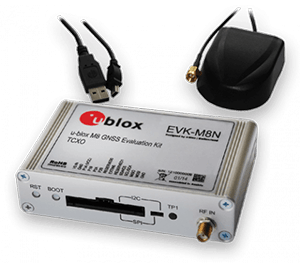
\includegraphics[width=1\textwidth]{imagenes/ublox.png}
	\caption{\label{fig1}U-blox EVK-M8F \cite{ublox}.}
\end{figure}

El dispositivo se conecta al ordenador mediante USB del que recibe la alimentación. A su vez se conecta una antena que debe situarse en algún espacio al aire libre en el que la recepción de la señal sea apropiada. La conexión por USB al ordenador proporciona al mismo tiempo los datos que se reciben. \newline

La empresa U-blox proporciona software para la correcta interacción con el dispositivo y los datos que este presta. U-center \cite{ucenter} es el software GNSS que soporta todos los dispositivos u-blox y permite visualizar e interactuar con los datos recibidos por este. Su interfaz gráfica permite visualizar los satélites de los que se recibe información, geolocalización, parámetros relacionados con la señal recibida, el tiempo, etc. La ventana de configuración permite indicar al dispositivo los mensajes que se quiere que este transmita. También se puede configurar la constelación de la que se quiere que el receptor reciba y envíe información. Los posibles datos a recibir se engloban en dos tipos, (1) NMEA (National Marine Electronics Association), estándar para la interacción con los dispositivos marinos electrónicos y (2) UBX, protocolo binario para los mensajes de posicionamiento. \newline

\begin{figure}
	\centering
	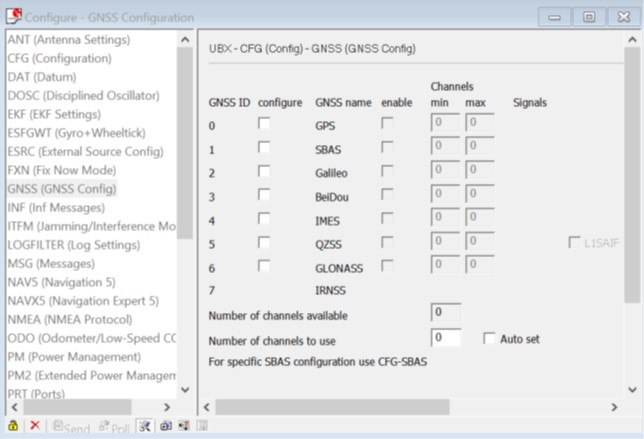
\includegraphics[width=1\textwidth]{imagenes/gnssconfig.jpg}
	\caption{\label{fig1}Configuración receptor U-blox desde u-center.}
\end{figure}

La información relevante para este trabajo se encuentra en los mensajes UBX-RXM-RAWX (Multi GNSS RAW Measurement Data). Estos mensajes lanzarán la información relacionada con el posicionamiento GNSS. Se activan por tanto estos mensajes y se procede al grabado de un fichero que contenga estos mensajes. Entre las herramientas se encuentra "Record" que permite generar un fichero en formato ublox que almacena estos mensajes durante tanto tiempo como se desee. Notar que los mensajes se encuentran en formato raw en este fichero. \newline

\begin{figure}
	\centering
	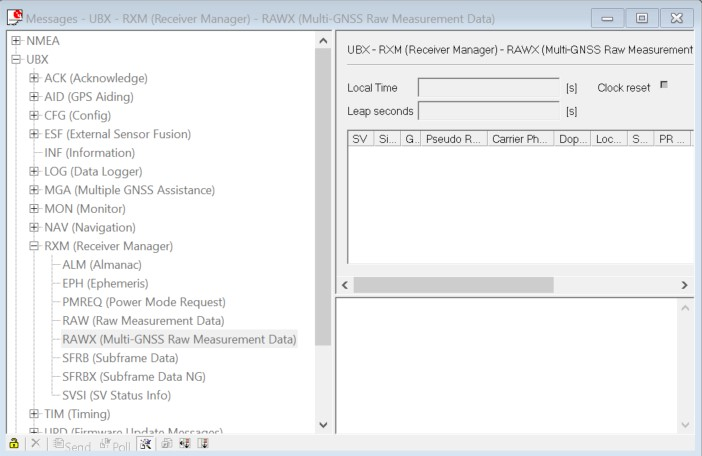
\includegraphics[width=1\textwidth]{imagenes/messagesview.jpg}
	\caption{\label{fig1}Ventana u-center para visualizar y habilitar mensajes.}
\end{figure}

\subsection{RTKLIB}
La librería de aplicaciones para el posicionamiento GNSS contiene una serie de aplicaciones para interactuar con todo lo relacionado con este sistema. \newline

En su repositorio de código \cite{reportklib} se encuentran los ejecutables de las distintas aplicaciones que ofrece. La aplicación CONVBIN permite convertir ficheros en diversos formatos a ficheros RINEX. Los ficheros generados en el apartado anterior sirven de entrada para esta aplicación. A la aplicación es necesario indicarle tanto el formato de entrada de los ficheros (ubx) como las salidas que se quiere que proporcione (ficheros de observaciones y de navegación).

La llamada a la aplicación se realiza por la terminal con el siguiente formato:

\begin{lstlisting}
>> ./convbin.exe -r ubx ./rawData.ubx -o file.obs -n file.nav -g file.gnav
\end{lstlisting}

Una ejecución exitosa de la aplicación nos genera los ficheros necesarios para las próximas tareas.

\subsection{Otros ficheros RINEX disponibles}
Existen muchos grupos que proporcionan de manera abierta todos los ficheros RINEX que graban. Uno de estos grupos es el Royal Observatory of Belgium que almacena todos sus ficheros RINEX en un servidor FTP \cite{ftprob} para que se puedan descargar de manera libre. \newline

Se tiene en cuenta esta posibilidad ya que como se verá en el apartado de "Generación de ficheros CGGTTS", no todos los ficheros RINEX son válidos para generar un CGGTTS.\newline


\section{Generación de ficheros CGGTTS}
El fichero CGGTTS contiene la información relacionada con la trazabilidad de tiempo del espacio temporal del que se tiene el fichero RINEX de un determinado dispositivo. \newline

El software encargado de generar ficheros CGGTTS a partir de ficheros RINEX se llama R2CGGTTS. Este software es desarrollado, mantenido y distribuido por el grupo Royal Observatory of Belgium. Esta herramienta está disponible en el FTP del BIPM \cite{ftpr2cggtts}. \newline

Al descargar la herramienta se observa que existen varias versiones de la misma. Durante los primeros meses de trabajo, la última versión disponible era la 7, así que al principio se trabaja con estas. En la documentación disponible para cada versión se observan las novedades que ha ido incluyendo cada una. Los aspectos más relevantes a tener en cuenta son la versión del fichero RINEX y las constelaciones GNSS que son soportadas. \newline

Para comenzar a trabajar con la herramienta el primer paso consiste en compilar el código con un compilador Fortran 77. 

\begin{lstlisting}
>> gfortran R2CGGTTS_V7.f -o R2CGGTTS_executable
\end{lstlisting}

Una vez compilado y generado el ejecutable, ya está listo para su ejecución. Antes de ejecutarlo hay que tener en cuenta que (1) los ficheros RINEX se deben colocar en el mismo directorio que el ejecutable y (2) se deben rellenar dos ficheros especiales (paramCGGTTS.dat e inputFile.dat). Estos dos ficheros contienen los parámetros relacionados con el receptor y los nombres de los ficheros RINEX de entrada. Ahora ya se puede ejecutar el código. Desde una terminal habrá que desplazarse al directorio correspondiente y lanzar el ejecutable.

\begin{lstlisting}
>> ./R2CGGTTS_executable
\end{lstlisting}

La salida esperada tras una ejecución exitosa es la creación en el mismo directorio de los ficheros CGGTTS.

\subsection{Problemas con la herramienta}
Pese a que fueron varios los problemas acontecidos durante el trabajo, hay dos que son los más representativos y que merece la pena mencionar.

\subsubsection{Versión del fichero RINEX}
Cada versión nueva del software R2CGGTTS ha ido incluyendo novedades a lo largo del tiempo. Una de ellas fue el cambio de versión (de la versión 2.x a la 3.x) de los ficheros RINEX entre las versiones 5 y 7 de la herramienta. El procedimiento seguido para generar un fichero RINEX (descrito en el apartado "Generación de ficheros RINEX") genera un fichero RINEX de versión 2.11. Esta versión es soportada solamente por la versión 5 del software R2CGGTTS. En paralelo a esto se prueba la versión 7 de R2CGGTTS con ficheros RINEX versión 3 disponibles online para su descarga.  \newline

En este tiempo se hace uso de herramientas que permiten la conversión de versiones de los ficheros RINEX \cite{gnssconverter}. Algunas de estas herramientas también permiten la conversión de ficheros raw en formato ublox a la versión deseada de fichero RINEX. Sin embargo, de ninguna herramienta se obtiene la salida esperada. \newline

Durante este tiempo de trabajo aparece la versión 8 del software R2CGGTTS. Entre las novedades que incluye, la principal consiste en permitir todas las versiones de ficheros RINEX. Cuando se subsana este problema aparece el siguiente que merece la pena mencionar.

\subsubsection{Requisito GPS P1 code o fichero biasC1P1.dat}
En la documentación, en el apartado de ficheros de entrada aparece un requisito: "\textit{biasC1P1.dat :Nedded if GPS P1 code is missing in Rinex observation file}". En caso de que el fichero RINEX no disponga de esa información, se necesitará un fichero adicional. \newline

Tras investigar sobre el tema, se llega a la conclusión de que la información \textit{GPS P1 code} es dependiente del receptor. Con el receptor U-blox XXXXXXXXXXXXXJoseLUis no es posible crear un RINEX que contenga esta información, sólo ciertos receptores lo permiten. \newline

XXXXXXXXXXLista de receptores P1XXXXXXX \newline

En el apartado "Generación de ficheros RINEX" se menciona un servidor FTP en el que el ROB almacena diariamente sus ficheros RINEX de manera que estén disponibles para su descarga. Los receptores utilizados por este grupo son bastante más avanzados y permiten crear ficheros RINEX con toda la información necesaria. Como plan alternativo, se hace uso de estos fichero RINEX para comprobar que efectivamente con esos ficheros el software R2CGGTTS se ejecuta satisfactoriamente y genera los ficheros CGGTTS esperados.


